% Construction : les courbes de exp et de ln, symétriques l'une de l'autre par
% rapport à la première bissectrice, tracée en pointillés.
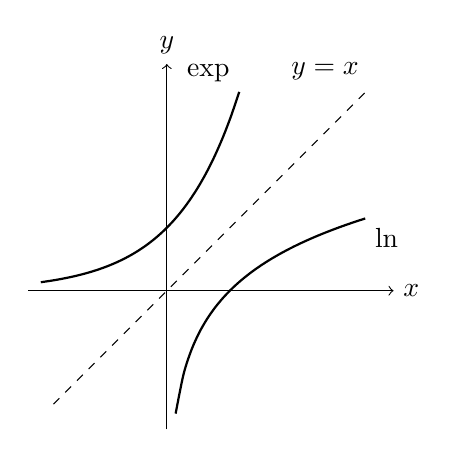
\begin{tikzpicture}[scale=0.8]
  \draw[->] (-2.2, 0) -- (3.6, 0) node[right] {$x$};
  \draw[->] (0, -2.2) -- (0, 3.6) node[above] {$y$};
  \draw[dashed] (-1.8, -1.8) -- (3.2, 3.2);
  \draw[thick, domain=-2:1.15, smooth, variable=\x] plot ({\x}, {exp(\x)});
  \draw[thick, domain=0.14:3.15, smooth, variable=\x] plot ({\x}, {ln(\x)});
  \node[above left] at (1.15, 3.16) {$\exp$};
  \node[below right] at (3.15, 1.15) {$\ln$};
  \node[above left] at (3.2, 3.2) {$y = x$};
\end{tikzpicture}
